การออกแบบทางโครงสร้างทางกลนั้น ผู้วิจัยได้เลือกใช้โปรแกรม Solidworks เป็นเครื่องมือที่ช่วยในการพัฒนาโมเดลของหุ่นยนต์ฮิวมานอยด์
เนื่องจากโปรแกรม Solidworks เป็นโปรแกรมที่มีความสามารถในการขึ้นรูปและวาดแบบทางวิศวกรรม
สามารถวิเคราะห์โครงสร้างทางกลของแบบจำลองได้ และมีการใช้งานอย่างแพร่หลาย อีกทั้งยังสามารถดาวน์โหลดโมเดลต่างๆ
ที่มีคนพัฒนาเข้าเข้ามาใช้ร่วมกับการออกแบบของเราได้ และด้วยทางผู้วิจัยมีความคำนึงถึงความสามารถในการพัฒนาต่อยอดเป็นหลัก
ดังนั้นการออกโครงสร้างทางกลของหุ่นยนต์ฮิวมานอยด์ UTHAI จึงถูกออกแบบมาเพื่อให้สามารถรองรับการเปลี่ยนแปลง
แก้ไขส่วนต่างๆของตัวหุ่นยนต์เองได้ในอนาคตอีกด้วย

\clearpage
\subsection{โครงสร้างหุ่นยนต์}
หุ่นยนต์ที่สร้างขึ้นประกอบด้วยส่วนของลำตัวและส่วนขา ในขาแต่ละข้างออกแบบให้เป็นลักษณะของข้อต่อหมุน (Revolute joint)
เลียนแบบโครงสร้างของมนุษย์ซึ่งประกอบด้วย ส่วนของสะโพกที่มีองศาอิสระจำนวน 3 องศาอิสระ ส่วนของหัวเข่า 1
องศาอิสระและส่วนของข้อเท้า 2 องศาอิสระ รวมขาข้างละ 6 องศาอิสระ ระบบต้นกำลังที่ใช้เป็น Dynamixel servo การออกแบบหุ่นยนต์นั้น
สิ่งแรกที่ต้องทำ คือ การกำหนดโครงสร้างของข้อต่อและก้านต่อขึ้นมาก่อน โดยวาดขึ้นมาเป็นเหมือนโครงกระดูก
ซึ่งโครงสร้างนั้นทางผู้วิจัยได้อ้างอิงมาจากสัดส่วนของมนุษย์จริง ที่ประกอบด้วยส่วนของขาข้างละ 6 องศาอิสระ และมีจุด CoM
อยู่บริเวณกระดูกเชิงกรานของตัวหุ่นยนต์เอง
\begin{figure}[!ht]
    \centering
    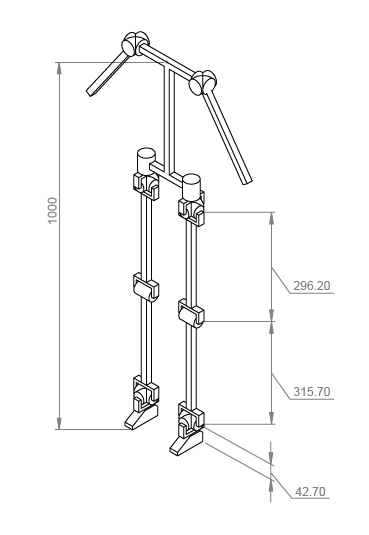
\includegraphics[width=0.35\textwidth]{chapter3/images/uthai_structure1.png}
    \caption{ภาพแสดงแสดงโครงสร้างของหุ่นยนต์ UTHAI}
    \label{fig:uthai_structure1}
\end{figure}

เมื่อเราได้แบบจำลองของหุ่นยนต์ฮิวมานอยด์ออกมาแล้ว ลำดับต่อไปคือการกำหนดตำแหน่งการติดตั้งเซนเซอร์และตัวขับเคลื่อนต่างๆเข้าไป
โดยมี Ground contact sensor ติดตั้งที่ใต้ฝ่าเท้าของหุ่นยนต์, IMU sensor ติดตั้งไว้ให้ใกล้กับจุด COM ของหุ่นยนต์ และ Dynamixel servo
ติดตั้งไว้ที่ข้อต่อในแต่ละข้อต่อ

\begin{figure}[!ht]
    \centering
    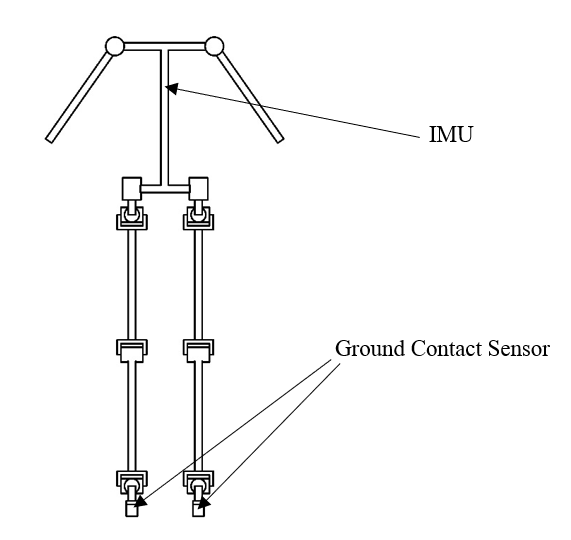
\includegraphics[width=0.5\textwidth]{chapter3/images/uthai_sensor.PNG}
    \caption{ภาพแสดงการติดตั้งเซนเซอร์ในจุดต่างๆ}
    \label{fig:uthai_structure2}
\end{figure}

ส่วนโครงสร้างหุ่นยนต์ฮิวมานอยด์ UTHAI ทางผู้วิจัยเลือกใช้วัสดุหลักเป็น PLA ที่ขึ้นรูปด้วยวิธีการขึ้นรูปสามมิติ
และมีวัสดุเสริมบางชิ้นส่วนจากอลูมิเนียม เนื่องจากจะทำให้โครงสร้างมีน้ำหนักเบา สามารถปรับปรุงแก้ไขง่าย และมีราคาที่สมเหตุสมผล
\begin{table}[ht]
	\centering
	\begin{tabular}{| l | l | l |}
		\hline
		Material & Longitudinal Tensile Strength ($ksi$) & Density ($g/cm^3$) \\
        \hline
        Carbon Fiber & 300 & 1.55 \\
        Steel & 100	& 7.7 \\
        Titanium & 120 & 4.34 \\
        Aluminum & 35 & 2.7 \\
        PLA 3D printing (50 \% infill) & 3.5 & 1.26 \\
        PLA 3D printing (100 \% infill) & 5.5 & 1.26 \\
	    \hline
	\end{tabular}
	\caption{ตารางแสดงสมบัติทางกลของวัสดุต่าง ๆ}
	\label{tab:material_properties}
\end{table}

\clearpage
\subsection{จัดทำชิ้นส่วนโครงสร้างและประกอบ}
ในกาารจัดทำชิ้นส่วนโครงสร้างนั้นทางผู้จัดทำได้คำนึงถึงความแข็งแรงเป็นหลักซึ่งมีความสำคัญมาก
ในการเคลื่อนที่ของหุ่นยนต์ และยังคงต้องมีน้ำหนักที่เบาอีกด้วย\footnote{ Printing Guide [https://filaments.ca/pages/temperature-guide]}
ดังนั้นจึงได้ใช้การขึ้นรูปชิ้นงานด้วยเทคนิค
การพิมพ์ 3 มิติ โดยจะใช้วัสดุหลักเป็นพลาสติก PLA ซึ่งมีความแข็งมากกว่าและขึ้นรูปง่ายกว่าพลาสติกชนิด ABS
เพื่อให้ตอบโจทย์กับหุ่นยนต์แพลตฟอร์มเพื่อพัฒนาต่อยอดในอนาคต ซึ่งผู้ใช้ทุกคนสามารถพิมพ์ขึ้นมาได้ด้วยตนเอง\footnote{ PLA vs ABS [https://www.3dhubs.com/knowledge-base/pla-vs-abs-whats-difference]}

\begin{table}[ht]
	\centering
	\begin{tabular}{| l | l | l |}
		\hline
		Properties & ABS & PLA \\
        \hline
        Tensile Strength & 27 $MPa$ & 37 $MPa$ \\
        Elongation & 3.5 \- 50\% & 6\% \\
        Flexural Modulus & 2.1 \- 7.6 $GPa$ & 4 $GPa$ \\
        Density & 1.0 - 1.4 $g/cm^3$ & 1.3 $g/cm^3$ \\
        Melting Point & 230$°C$ - 240$°C$ & 215$°C$ - 235$°C$ \\ 
        การย่อยสลายทางธรรมชาติ & ไม่ได้ & ได้(ภายใต้เงื่อนไขที่ถูกต้อง) \\
	    \hline
	\end{tabular}
	\caption{ตารางแสดงสมบัติทางกลของวัสดุพลาสติก}
	\label{tab:plastic_material_properties}
\end{table}
แต่เนื่องจากว่าในปัจจุบันนี้เครื่องพิมพ์ส่วนมากจะไม่รองรับการพิมพ์ชิ้นงานที่มีขนาดใหญ่ ซึ่งมีขนากมากกว่า
30x30x30 ซม.(กว้างxยาวxสูง) ดังนั้นชิ้นงานที่ขึ้นรูปที่มีขนาดใหญ่เกินกว่านี้อาจจะต้องทำการตัดชิ้นงานออกก่อน
แล้วจึงค่อยนำมาประกอบรวมกันทีหลังอีกครั้งหนึ่ง โดยพื้นที่ทำการพิมพ์ของเครื่องพิมพ์ 3 มิติที่มีวางจำหน่าย
และใช้งานแพร่หลายในท้องตลาดแสดงดังตาราง\ref{tab:3dprint_space} \footnote{The truth about 3D printer maximum print areas [https://www.zdnet.com/article/what-manufacturers-dont-want-you-to-know-the-truth-about-3d-printer-maximum-print-areas/]}

\begin{table}[ht]
	\centering
	\begin{tabular}{| l | l | l | l |}
		\hline
		Printer & Actual Width & Actual Depth & Actual Height \\
        \hline
        MakerBot Replicator+ & 292 & 192 & 165 \\
        Ultimaker 3 & 188 & 185 & 200 \\
        LulzBot Mini & 152 & 152 & 158 \\
        Dreammaker Overlord Pro Plus & 79 & 79 & 255 \\
        New Matter MOD-t & 145 & 95 & 125 \\
	    \hline
	\end{tabular}
	\caption{ตารางแสดงขนาดของชิ้นงานที่สามารถพิมพ์ได้ในเครื่องพิมพ์ชนิดต่างๆ}
	\label{tab:3dprint_space}
\end{table}





%%%%%%%%%%%%%%%%%%%%%%%%%%%%%%%%%%%%%%%%%%%%%%%%%%%%%%%%%%%%%%%%%%%%%%%%%%%%%%%
%%%%%%%%%%%%%%%%%%%%%%%%%%%%%%%%%%%%%%%%%%%%%%%%%%%%%%%%%%%%%%%%%%%%%%%%%%%%%%%
%%%%%%%%%%%%%%%%%%%%%%%%%%%%%%%%%%%%%%%%%%%%%%%%%%%%%%%%%%%%%%%%%%%%%%%%%%%%%%%
\clearpage
\subsection{อุปกรณ์ที่ใช้ในหุ่นยนต์ฮิวมานอยด์อุทัย}

\subsubsection*{Dynamixel servo EX-106+}
Dynamixel EX-106+ เป็นตัวขับเคลื่อนที่นิยมใช้ในปัจจุบัน ซึ่งเป็นเซอร์โวมอเตอร์ที่เหมาะสำหรับทำหุ่นยนต์โดยเฉพาะ
ภายในประกอบไปด้วย มอเตอร์กระแสตรง ชุดเฟืองมอเตอร์ ไดรเวอร์คอนโทรเลอร์ สามารถเชื่อมต่อกันผ่าน BUS RS-485
\footnote{ Robot Actuator [http://support.robotis.com/en/product/actuator/dynamixel/ex\_series/ex-106.htm] }
มีการควบคุมแบบ PID สามารถที่จะอ่านค่าความเร็ว
แรงดันไฟฟ้า กระแสไฟฟ้า อุณหภูมิ ตำแหน่ง และแรงบิดจากมอเตอร์ทุกตัวได้ แต่ละมอเตอร์แต่ละตัวจะมีบอร์ดควบคุมของตัวเอง
เราสามารถที่จะจ่ายไฟให้มอเตอร์และควบคุมผ่าน Serial ได้เลย

การทำงานของตัวขับเคลื่อนนี้สามารถทำได้ 2 รูปแบบคือ\footnote{ EX-106+ Mode [http://www.trossenrobotics.com/dynamixel-ex-106-robot-actuator.aspx] }

\paragraph*{Joint Mode}
สามารถที่จะควบคุม Torque Speed และ position ได้ความละเอียดในการควบคุม 10-bit (0-1023) หมุนได้อยู่ในช่วง 0-250 องศา

\paragraph*{Wheel Mode}
สามารถที่จะควบคุม Torque Speed และ direction ได้ ความละเอียดของความเร็วมอเตอร์เท่ากับ 10bit (0-1023) สามารถหมุนได้ครบ 360 องศาได้

\begin{figure}[!ht]
    \centering
    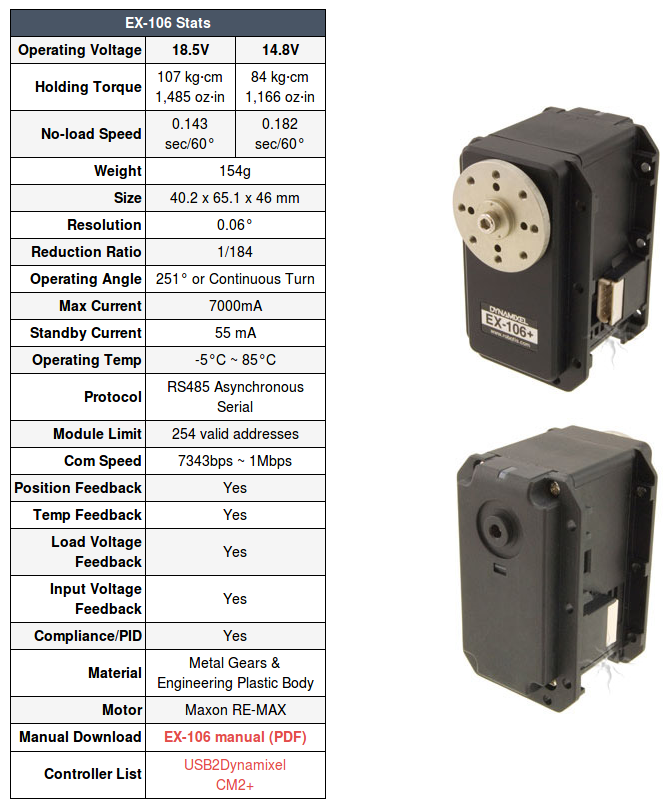
\includegraphics[width=0.75\textwidth]{chapter3/images/dxl_ex106.png}
    \caption{แสดงประสิทธิภาพของมอเตอร์ EX-106+}
    \label{fig:dxl_ex106}
\end{figure}


\clearpage
\subsubsection*{USB2Dynamixel connector}
USB2Dynamixel เป็นอุปกรณ์สำหรับเชื่อมต่อ Odroid กับ Dynamixel Motor
โดยจะเชื่อมต่อผ่านพอร์ท USB ของ Odroid ไปยัง Dynamixel motor
ผ่านสายทั้งหมด 2 เส้น คือ D+ และ D-
เป็นการเชื่อมต่อแบบ RS-485\footnote{USB2Dynamixel [http://support.robotis.com/en/product/auxdevice/interface/usb2dxl\_manual.html]}
ืทำให้สามารถส่งข้อมูลระยะทางไกลได้ และสามารถที่จะมีหลายอุปกรณ์บนสายเส้นเดียวกันได้

\begin{figure}[!ht]
    \centering
    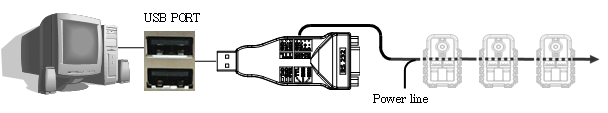
\includegraphics[width=0.75\textwidth]{chapter3/images/dynamixel2pc.png}
    \caption{ภาพแสดงการติดต่อสื่อสารระหว่าง PC กับมอเตอร์ Dynamixel}
    \label{fig:dynamixel2pc}
\end{figure}

ในการต่อใช้งานนั้นผู้ใช้งานจำเป็นต้องเลือกการติดต่อสื่อสารระหว่าง คอมพิวเตอร์กับมอเตอร์
ซึ่งการติดต่อสื่อสารนั้นหากใช้ USB2Dynamixel ตัวอุปกรณ์ชิ้นนี้ได้แบ่งการติดต่อสื่อสารออกเป็น 3 รูปแบบคือ
\vspace{-10pt}
\begin{enumerate}[label=\arabic*, leftmargin=1.5cm]
    \setlength\itemsep{-0.25em}
    \item TTL Communication : สำหรับมอเตอร์ Dynamixels ที่ใช้พอร์ทชนิด 3-pin เช่นในตระกูล AX Series เช่น AX-S1 AX-12+ ฯลฯ
    \item RS485 Communication : สำหรับมอเตอร์ Dynamixels ที่ใช้พอร์ทชนิด 4-pin เช่นในตระกูล DX Series เช่น RX Series, EX Series ฯลฯ
    \item RS232 Communication : ใช้สำหรับติดต่อสื่อสารกับคอนโทรลเลอร์ผ่านสายเคเบิล
\end{enumerate}
\vspace{-15pt}
\begin{figure}[!ht]
    \centering
    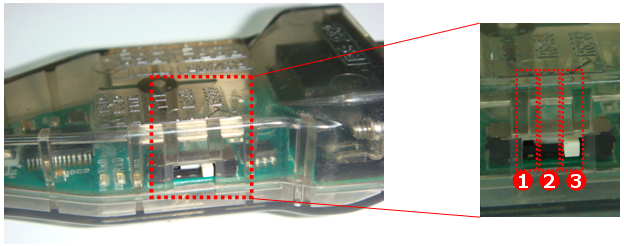
\includegraphics[width=0.5\textwidth]{chapter3/images/useusb2dynamixel.png}
    \caption{ภาพแสดงการเลือกโหมดใช้งานของ USB2Dynamixel}
    \label{fig:useusb2dynamixel}
\end{figure}

แต่จากการทดลองนำมาใช้ผู้วิจัยพบว่า Dynamixels ที่ใช้ในการทำงานวิจัยครั้งนี้เป็นชนิด 4 pin ซึ่งใช้ RS485 ในการติดต่อสื่อสาร
และด้วยขนาดของตัว USB2Dynamixel มีขนาดที่ใหญ่ทำให้การทำงานมีความลำบากในการติดตั้งลงบนตัวของหุ่นยนต์
จึงได้ทำการเปลี่ยนเป็น USB to RS485 แทน
\begin{figure}[!ht]
    \centering
    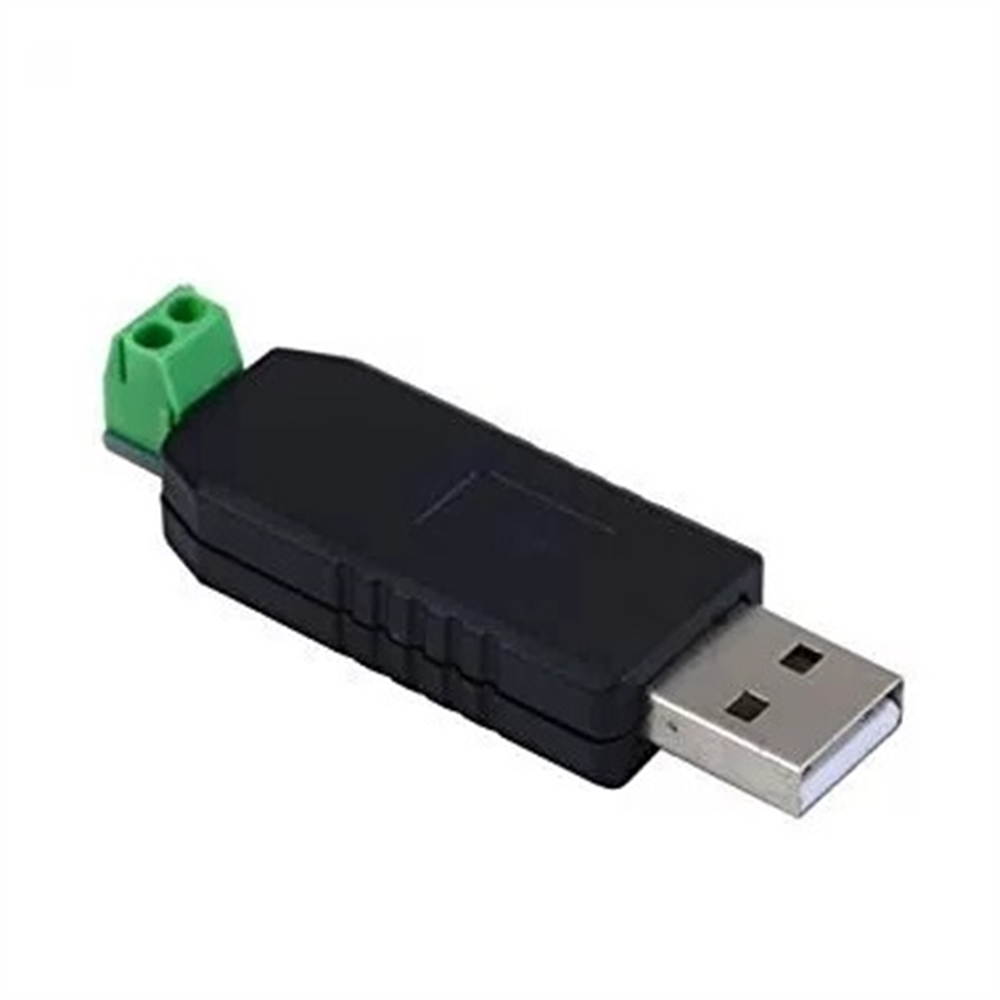
\includegraphics[width=0.3\textwidth]{chapter3/images/usb2rs485.jpg}
    \caption{USB2RS485 Module}
    \label{fig:usb2rs485}
\end{figure}

\clearpage
\subsubsection*{Inertial Measurement Unit (IMU)}
ในการทำวิจัยครั้งนี้ผู้จัดทำได้เลือกนำเซนเซอร์ MPU-9250 มาใช้ในการอ่านค่ามุมเอียงของหุ่นยนต์เพื่อใช้ในการคุมเสถียรภาพของหุ่นยนต์
โดยเซนเซอร์ตัวนี้สามารถวัดค่าได้ 9 แกนคือ วัดค่าความเร็วเชิงมุม(gyroscope) 3 แกน วัดค่าความเร่งเชิงเส้น(accelerometer) 3 แกน
และวัดค่าสนามแม่เหล็กโลก({magnetometer) 3 แกน ซึ่งเซนเซอร์ตัวนี้จะติดตั้งบริเวณส่วนของลำตัวหุ่นยนต์
เนื่องจากว่าจะเป็นจุดที่สามารถบ่งบอกได้ถึงการเคลื่อนที่และมุมเอียงของหุ่นยนต์ในขณะนั้นได้ดีที่สุด\footnote{ MPU-9250 [http://www.arduiner.com/en/gy-series-axis-accellerometers/6924-gy9255-mpu9255-sensor-module-alternative-mpu9150-mpu9250-3809200640200.html] }
\begin{figure}[!ht]
    \centering
    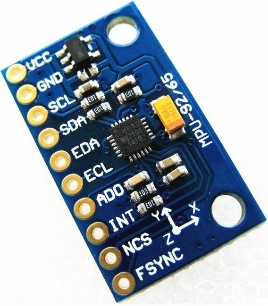
\includegraphics[width=0.2\textwidth]{chapter3/images/mpu9250.jpeg}
    \caption{แสดงเซนเซอร์ IMU MPU9250}
    \label{fig:mpu9250}
\end{figure}

\subsubsection*{Wi-Fi Adapter}
ตัวรับสัญญาณ wifi ชนิดพกพาเพื่อใช้ในการติดต่อสื่อสารระหว่างคอมพิวเตอร์ที่ติดตั้งอยู่บนตัวของหุ่นยนต์
และคอมพิวเตอร์ที่เป็นตัวสั่งการซึ่งอยู่นอกตัวของหุ่นยนต์ ซึ่งในงานวิจัยนี้
จะใช้ส่งข้อมูลที่ได้หลังจากการประมวลผลบนคอมพิวเตอร์ไปยังตัวหุ่นยนต์ เช่น การวางแผนการเดิน การคำนวนพลศาสตร์ของหุ่นยนต์
และอื่นๆ โดยการส่งข้อมูลไปยังคอมพิวเตอร์ที่อยู่บนตัวหุ่นยนต์นั้นจะมีตัวกลางในการรับส่งสัญญาณ
คือ ตัวกระจายสัญญาณ (wifi router)
\begin{figure}[!ht]
    \centering
    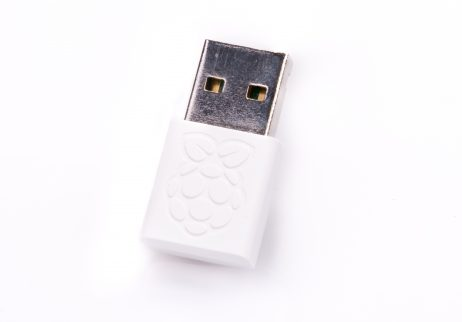
\includegraphics[width=0.3\textwidth]{chapter3/images/rpi_wifi_adaptor.jpg}
    \caption{ตัวรับสัญญาณ wifi ของ RaspberryPi}
    \label{fig:rpi_wifi_adaptor}
\end{figure}
\begin{figure}[!ht]
    \centering
    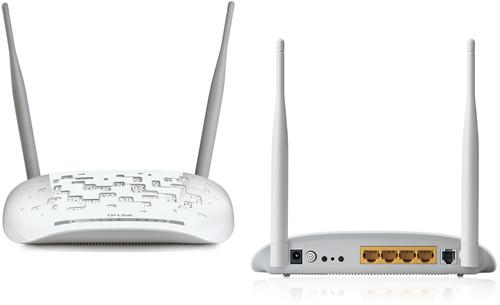
\includegraphics[width=0.3\textwidth]{chapter3/images/wifi_router.jpg}
    \caption{ตัวกระจายและรับส่งสัญญาณ wifi}
    \label{fig:wifi_router}
\end{figure}


\clearpage
\subsubsection*{Ground contact sensor}
เซนเซอร์ตรวจหน้าสัมผัสที่พื้นเป็นเซนเซอร์ที่ถูกติดตั้งบริเวณฝ่าเท้า เพื่อตรวจสอบการเดินของหุ่นยนต์ฮิวมานอยด์ว่าขณะนี้มีการสัมผัสของฝ่าเท้าของหุ่นยนต์กับพื้นหรือไม่ 
ซึ่งในงานวิจัยนี้ได้ใช้หลักการตัวตรวจจับแรงกดแบบค่าความต้านทานหรือ Force Sensing Resistor (FSR) ที่ใช้เทคโนโลยีฟิล์มโพลีเมอร์แบบหนา (Polymer Thick Film) 
โดยแรงดันไฟฟ้าที่ตกคร่อมตัวตรวจจับจะลดลง เมื่อมีแรงกดมากระทำบนแผ่นตรวจจับ มีโครงสร้างของตัวตรวจจับแสดง ดังรูปที่ \ref{fig:FSRarchitec}
\begin{figure}[!ht]
    \centering
    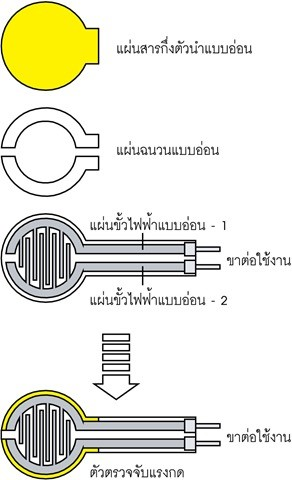
\includegraphics[width=0.35\textwidth]{chapter3/images/FSRarchitec.jpg}
    \caption{ลักษณะโครงสร้างของตัวตรวจจับแรงกด FSR}
    \label{fig:FSRarchitec}
\end{figure}

ประกอบด้วยแผ่นสารกึ่งตัวนำแบบอ่อนที่เป็นตัวกำหนดค่าความต้านทานไฟฟ้าประกบ เข้ากับแผ่นขั้วไฟฟ้าแบบอ่อน โดยมีแผ่นฉนวนแบบอ่อนคั่นกลาง 
ทำให้เกิดค่าความต้านทานไฟฟ้าขึ้นระหว่างขาต่อใช้งาน เมื่อมีการกดลงบนแผ่นขั้วนำไฟฟ้า จะทำให้เกิดการสัมผัสระหว่างสารกึ่งตัวนำกับขั้วไฟฟ้า
ส่งผลให้ค่าความต้านทานไฟฟ้าเกิดการเปลี่ยนแปลง ดังแสดงกระบวนการทำงานในรูปที่ \ref{fig:FSRfunction}
\begin{figure}[!ht]
    \centering
    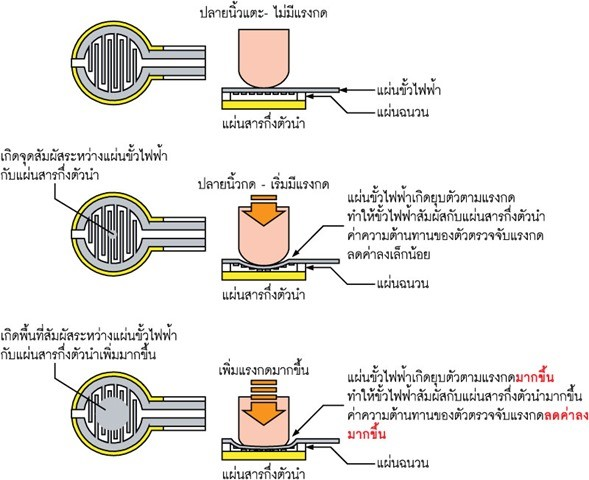
\includegraphics[width=0.5\textwidth]{chapter3/images/FSRfunction.jpg}
    \caption{การทำงานของตัวตรวจจับแรงกด FSR}
    \label{fig:FSRfunction}
\end{figure}

แนวคิดการออกแบบหลัก คือการออกแบบให้สามารถติดตั้งกับตัวหุ่นยนต์ได้เลย ไม่ต้องเชื่อมต่อสายไฟและสายส่งข้อมูลใหม่ โดยให้ใช้สายไฟไฟเลี้ยง 
และสายสัญญาณชุดเดียวกับตัวขับเคลื่อน Dynamixel Servo Mo-tor ซึ่งมีการติดต่อกันในลักษณะเป็นบัสแบบ RS-485 ดังนั้นแล้วผู้เขียนจึงเลือกที่จะทำโมดูลขึ้นมาใหม่ 1 โมดูล 
เพื่อที่ใช้ในการอ่านค่า Ground Contact Sensor ของหุ่นยนต์โดยเฉพาะ โดยมีการติดต่อรูปแบบบัส RS-485 ใช้ลักษณะการติดต่อสื่อสาร(Protocol) เดียวกับตัวขับเคลื่อน Dynamixel 
และมีการพัฒนาจาก Arduino ซึ่งให้สามารถอ่านค่าได้ทั้ง Analog และ Digital ได้ อีกทั้งรองรับการต่อ Sensor แบบ Force sensitive resistor จำนวน 4 ตัว.
\begin{figure}[!ht]
  \centering
  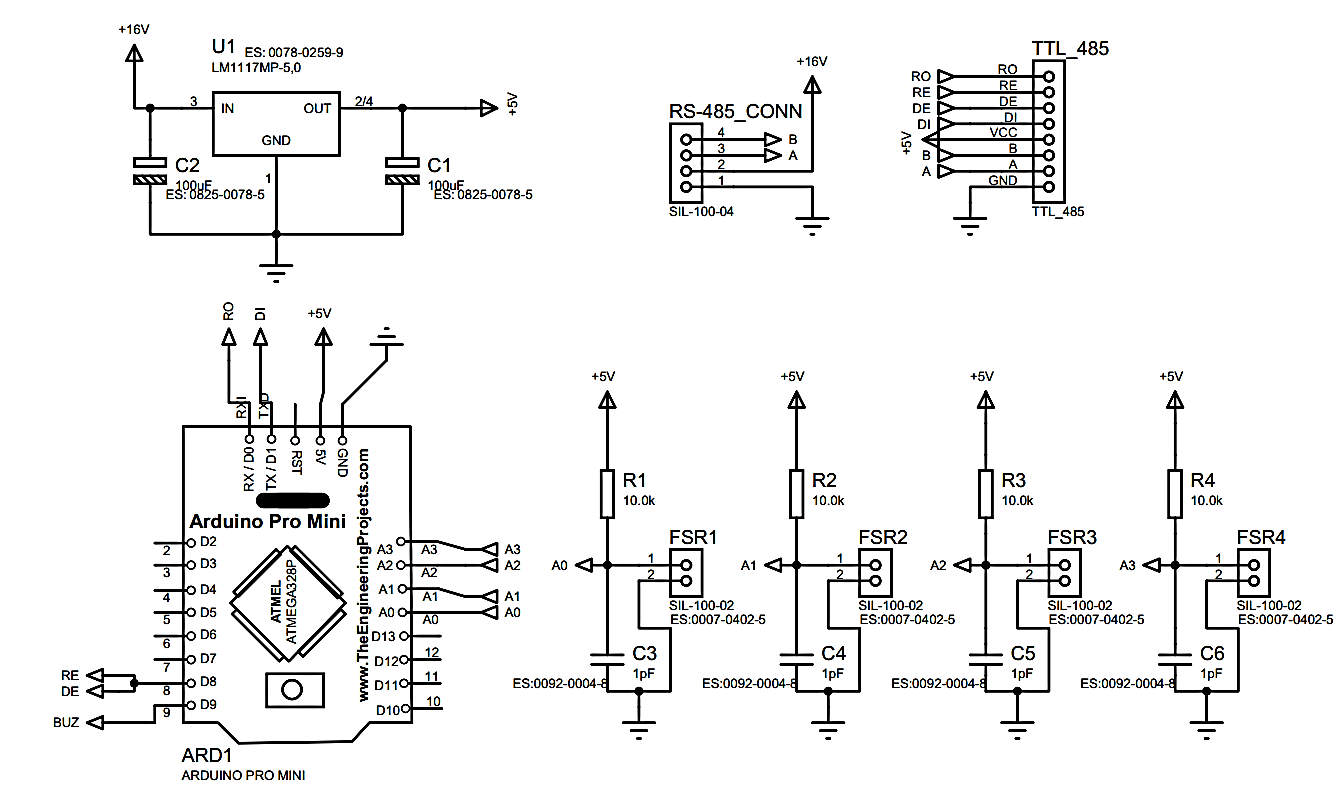
\includegraphics[width=0.8\textwidth]{chapter3/images/FSR_schematic.png}
  \caption{Schematic ของวงจร Ground Contact Sensor}
  \label{fig:FSR_schematic}
\end{figure}

\begin{figure}[!ht]
  \centering
  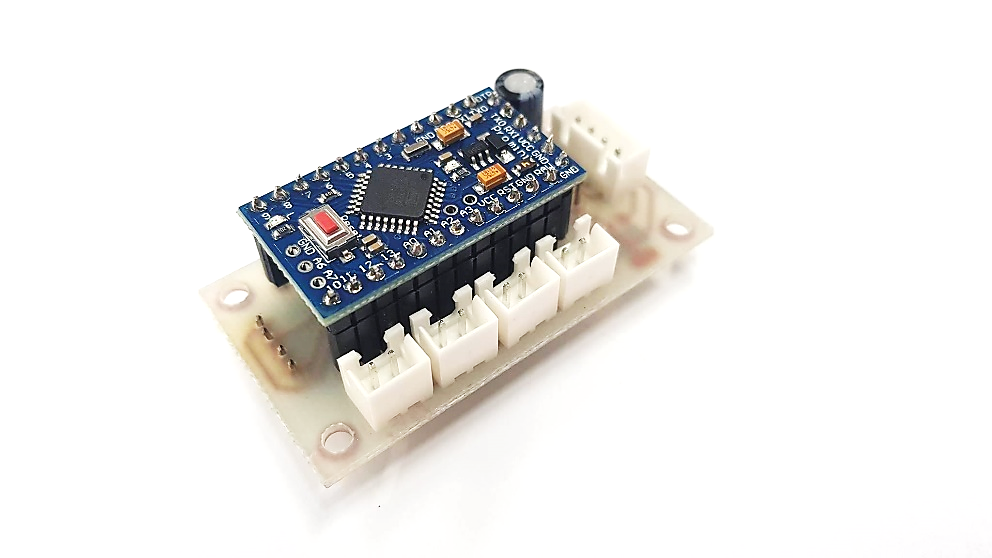
\includegraphics[width=0.8\textwidth]{chapter3/images/complete_FSR.png}
  \caption{แผงวงจร Ground Contact Sensor ที่ประกอบเสร็จแล้ว}
  \label{fig:complete_FSR}
\end{figure}

\clearpage
เซนเซอร์ที่เลือกใช้คือ Force Sensitive Resistor (FSR) เป็นเซนเซอร์ที่มีค่าความต้านทานภายในตัวเอง โดยเซนเซอร์นี้มีหลักการทำงานคือ 
ค่าความต้านทานทางไฟฟ้าของตัวเซนเซอร์จะเปลี่ยนแปลงเมื่อมีแรงเข้ามากระทำกับหน้าสัมผัส เมื่อมีแรงเข้ามากระทำมาก จะทำให้ค่าความต้านทานต่ำ 
หากไม่มีแรงเข้ามากระทำจะทำให้มีค่าความต้านทานสูง และเมื่อมีการนำเซนเซอร์นี้มาต่อกับตัวต้านทานที่มีค่าคงที่ ในรูปแบบของ Voltage Divider 
ดังรูปที่ \ref{fig:FSR_schematic} จะทำให้สามารถอ่านค่าแรงดันไฟฟ้าที่เปลี่ยนแปลงตามแรงที่เกิดขึ้นกับหน้าสัมผัสของเซนเซอร์ FSR ได้ 

\begin{figure}[!ht]
  \centering
  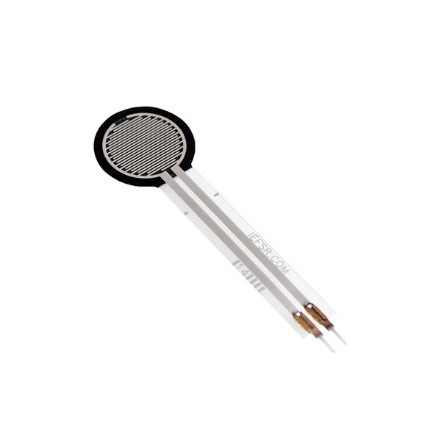
\includegraphics[width=0.3\textwidth]{chapter3/images/FSR.jpg}
  \caption{Force Sensitive Resistor (FSR) ขนาด 0.5 นิ้ว}
  \label{fig:FSR}
\end{figure}

ข้อดีของ FSR นั้นคือ เป็นเซนเซอร์ที่ถูกพัฒนาและออกแบบมาเพื่อใช้สำหรับการวัดแรงโดยตรง จึงทำให้ใช้งานได้ง่าย และสะดวก ในราคาที่ถูกกว่า 
เมื่อเทียบกับเซนเซอร์ Load cell ที่มีราคาสูงและการใช้งานจำเป็นที่จะต้องมีวงจรขยายสัญญาณที่ใช้ในการอ่านค่าการบิดของวัสดุจาก 
แต่ FSR นั้นก็มีข้อเสียเช่นกันคือ ความไม่ทนทานต่อการขีดข่วน เนื่องจากตัวเซนเซอร์ถูกทำมาจากฟิล์มพลาสติกบางๆ ซึ่งหากเกิดการขีดข่วนเกิดขึ้นแล้วอาจทำให้ฟิล์มฉีกขาดได้ 
หากฟิล์มขาดจะทำให้ค่าความต้านทานออกมาไม่เหมือนเดิม ดังนั้นทางผู้เขียนจึงเลือกที่จะออกแบบโครงครอบสำหรับเซนเซอร์ FSR เพื่อป้องกันจากการถูกขีดข่วนจากภายนอก







%%%%%%%%%%%%%%%%%%%%%%%%%%%%%%%%%%%%%%%%%%%%%%%%%%%%%%%%%%%%%%%%%%%%%%%%%%%%%%%
\clearpage
\subsection{การเชื่อมต่อตัวขับเคลื่อนและตัวรับรู้}
โครงสร้างของหุ่นยนต์ฮิวมานอยด์อุทัยจะมีขาสองข้างทำให้เกิดองศาอิสระ 12 องศาอิสระ
จึงใช้ดิจิตอลเซอร์โวทั้งหมด 12 ตัว ดิจิตอลเซอร์โวทุกตัวเชื่อมต่อกันแบบเดซี่เชน (daisy chain) ดังรูปที่ \ref{fig:dynamixel_connect}
ข้างนึงของมอเตอร์ตัวแรกเชื่อมต่อกับแบตเตอร์รี่ 12V และอีกข้างต่อกับ USB2RS485 เพื่อต่อไปยังตัวประมวลผระดับสูง (Odroid)
และเซนเซอร์หน่วยวัดความเฉื่อย กับเซนเซอร์ตรวจจับหน้าสัมผัสที่พื้นเชื่อมต่อกับตัวประมวลผลระดับต่ำ (Nucleo F411RE)
ดังรูปที่ \ref{fig:odroid2dynamixel}
\begin{figure}[!ht]
    \centering
    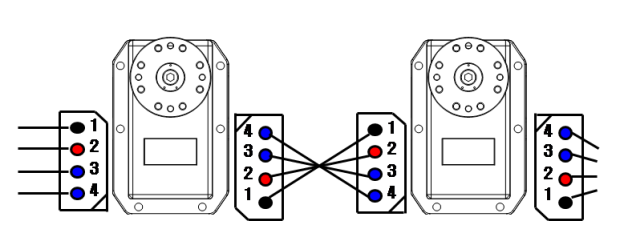
\includegraphics[width=0.7\textwidth]{chapter3/images/dynamixel_connect.png}
    \caption{การเชื่อมต่อกันระหว่างดิจิตอลเซอร์โว}
    \label{fig:dynamixel_connect}
\end{figure}
\begin{figure}[!ht]
    \centering
    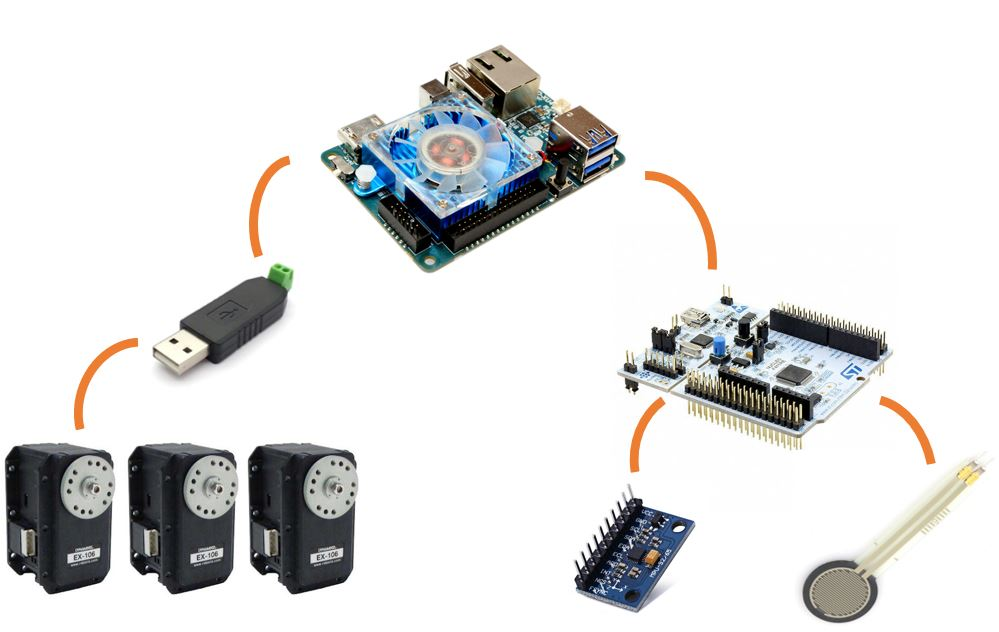
\includegraphics[width=0.9\textwidth]{chapter3/images/odroid2dynamixel.JPG}
    \caption{การเชื่อมต่อระหว่างตัวรับรู้ ตัวประมวลผล และตัวขับเคลื่อน}
    \label{fig:odroid2dynamixel}
\end{figure}


%%%%%%%%%%%%%%%%%%%%%%%%%%%%%%%%%%%%%%%%%%%%%%%%%%%%%%%%%%%%%%%%%%%%%%%%%%%%%%%
\clearpage
\subsection{การตั้งค่ามอเตอร์}

\begin{wrapfigure}{l}{0.2\textwidth}
    
\includegraphics[width=0.9\linewidth]{chapter3/images/roboplus/roboplus.jpg} 
    \caption*{Roboplus}
\end{wrapfigure}

หลังจากที่เราเชื่อมต่อมอเตอร์เข้ากับระบบแล้วก็ต้องมีการตั้งค่ามอเตอร์ก่อน โดยการตั้งค่ามอเตอร์นั้นจะใช้โปรแกรม
Roboplus เป็นเครื่องมือที่ช่วยให้เราสามารถติดต่อกับมอเตอร์ได้ แต่ใช้ได้เฉพาะใน Windows เท่านั้น ซึ่งสามารถดาวน์โหลดได้จากหน้าเว็บ Robotis
เมื่อเราดาวน์โหลดโปรแกรมและติดตั้งเรียบร้อยแล้ว ให้เชื่อมต่อมอเตอร์กับ USB2RS485 ทีละตัว และทำตามขั้นตอน ตามภาพ
\begin{figure}[!ht]
    \centering
    
\includegraphics[width=0.5\textwidth]{chapter3/images/roboplus/roboplus1.PNG}
    \caption*{ต่อมอเตอร์เข้ากับคอมพิวเตอร์ด้วย USB2RS485}
\end{figure}
\begin{figure}[!ht]
    \centering
    
\includegraphics[width=0.4\textwidth]{chapter3/images/roboplus/roboplus1.PNG}
    \caption*{ต่อมอเตอร์เข้ากับพาวเวอร์ซัพพลาย}
\end{figure}
\begin{figure}[!ht]
    \centering
    
\includegraphics[width=0.15\textwidth]{chapter3/images/roboplus/roboplus1.PNG}
    \caption*{เปิดโปรแกรม Roboplus ขึ้นมา}
\end{figure}
\begin{figure}[!ht]
    \centering
    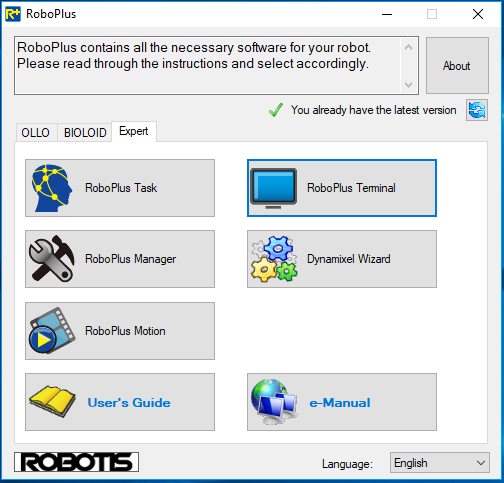
\includegraphics[width=0.55\textwidth]{chapter3/images/roboplus/roboplus2.PNG}
    \caption*{กดเข้าไปที่ Dynamixel Wizard}
\end{figure}
\begin{figure}[!ht]
    \centering
    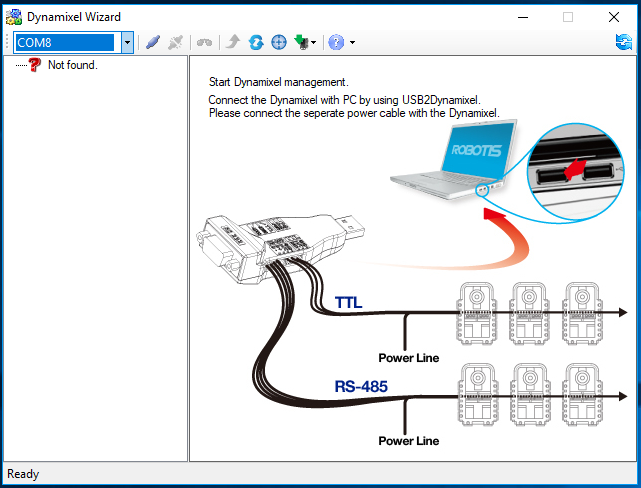
\includegraphics[width=0.55\textwidth]{chapter3/images/roboplus/roboplus3.PNG}
    \caption*{เลือก COM Port ให้ตรงกับ USB2RS485 จากนั้นกด Connect}
\end{figure}
\begin{figure}[!ht]
    \centering
    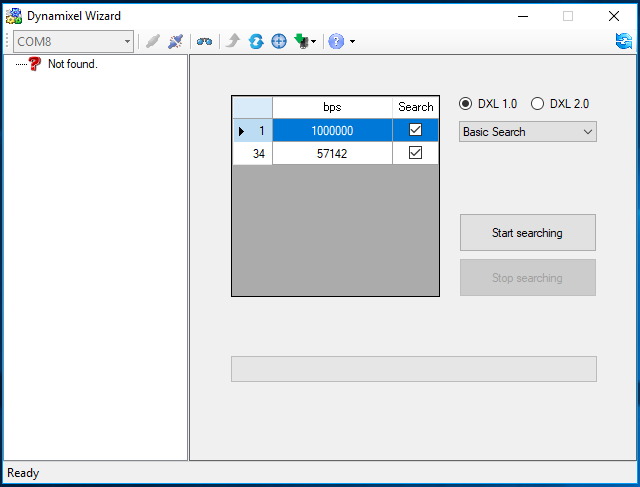
\includegraphics[width=0.55\textwidth]{chapter3/images/roboplus/roboplus4.PNG}
    \caption*{ติ๊กถูกที่ช่อง 1Mbps แล้วกด Start searching}
\end{figure}
\begin{figure}[!ht]
    \centering
    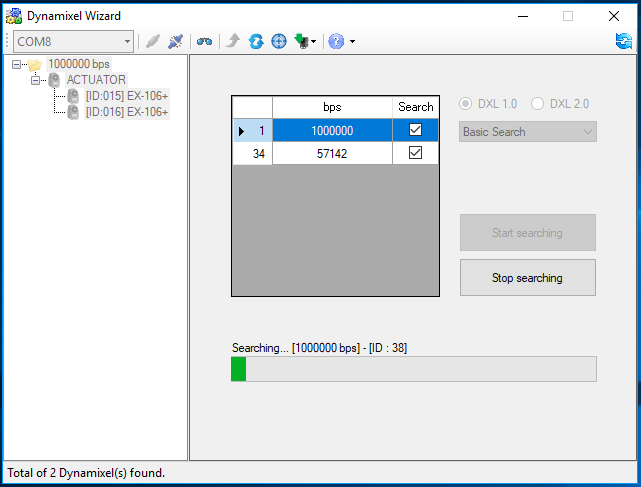
\includegraphics[width=0.55\textwidth]{chapter3/images/roboplus/roboplus5.PNG}
    \caption*{เมื่อเห็นทางด้านซ้ายมือโผล่ ID มอเตอร์ขึ้นมา หากขึ้นแล้วก็สามารถกด Stop Searching ได้}
\end{figure}
\begin{figure}[!ht]
    \centering
    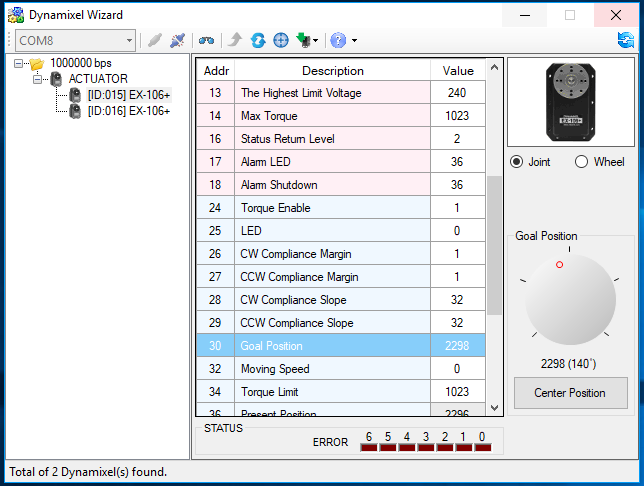
\includegraphics[width=0.55\textwidth]{chapter3/images/roboplus/roboplus6.PNG}
    \caption*{ทดสอบสั่งการมอเตอร์ที่ Addr 30 Goal position ว่าทิศทางถูกต้องหรือไม่}
\end{figure}
\begin{figure}[!ht]
    \centering
    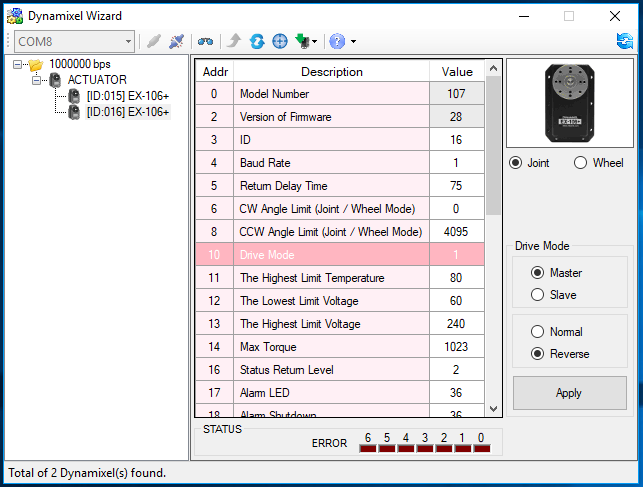
\includegraphics[width=0.55\textwidth]{chapter3/images/roboplus/roboplus7.PNG}
    \caption*{ถ้าทิศทางไม่ถูกต้องสามารถที่จะปรับได้ที่ Addr 10 Drive mode}
\end{figure}

%%%%%%%%%%%%%%%%%%%%%%%%%%%%%%%%%%%%%%%%%%%%%%%%%%%%%%%%%%%%%%%%%%%%%%%%%%%%%%%
\clearpage
\subsection{การเชื่อมต่อบอร์ดประมวลผล}
การเชื่อมต่อระหว่างบอร์ดประมวลผลระดับล่างกับบอร์ดประมวลผลระดับสูง โดยจะเชื่อมต่อกันผ่านสาย USB
และส่งข้อมูลหากันผ่าน Serial โดยใช้ ROSserial นอกจากจะมีบอร์ดประมวลผลแล้วยังมีบอร์ดที่เอาไว้ใช้สำหรับควบคุม
dynamixel servo เพื่อเผื่อเอาไว้สำหรับเปลี่ยนให้ ตัวประมวลผลควบคุมระดับล่างเป็นตัวสั่งการมอเตอร์
ดัวรูปที่ \ref{fig:uthai_controller}

\begin{figure}[!ht]
    \centering
    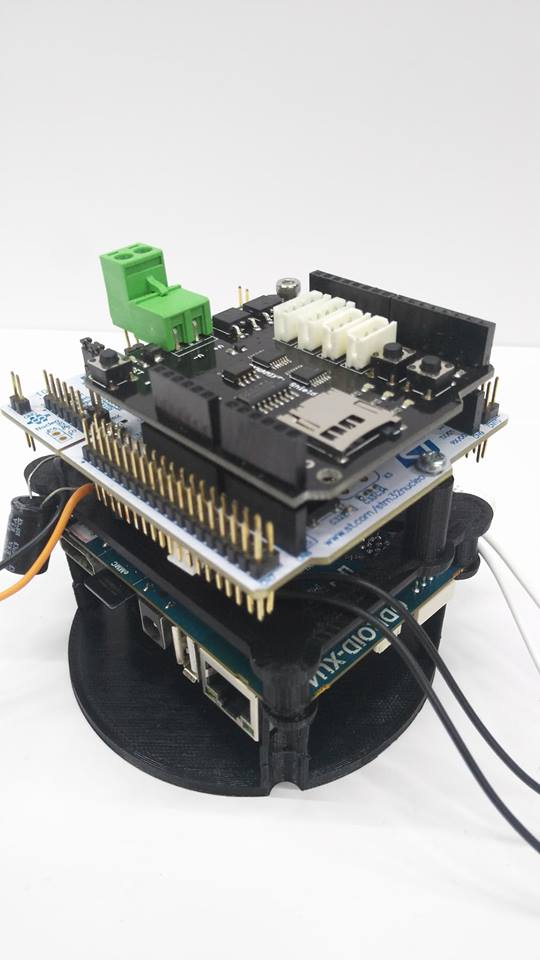
\includegraphics[width=0.4\textwidth]{chapter3/images/uthai_controller.jpg}
    \caption{การเชื่อมต่อกันระหว่างตัวประมวลผล}
    \label{fig:uthai_controller}
\end{figure}




\clearpage
\newcommand{\addprop}[9]{
	CoM X (m) & #1\\
	CoM Y (m) & #2\\
	CoM Z (m) & #3\\
	Inertia Ixx & #4\\
	Inertia Ixy & #5\\
	Inertia Ixz & #6\\
	Inertia Iyy & #7\\
	Inertia Iyz & #8\\
	Inertia Izz & #9\\
}

\subsection{Dynamic properties}
ข้อมูลพลศาสตร์ของหุ่นยนต์จะเอาไว้ใช้ในการทำ Simulation บนระบบ ROS และเอาไปใช้ในการคำนวณทางคณิตศาสตร์ได้
โดยข้อมูลนี้เอามาจาก SolidWorks แล้วปรับให้มีค่าใกล้เคียงกับของจริงมากที่สุด

ข้อมูลที่จำเป็นในการใช้งานจะประกอบไปด้วย มวล จุดศูนย์กลางมวล และโมเมนต์ความเฉื่อย

\subsubsection*{Overall Humanoid}
\begin{figure}[!ht]
	\centering
	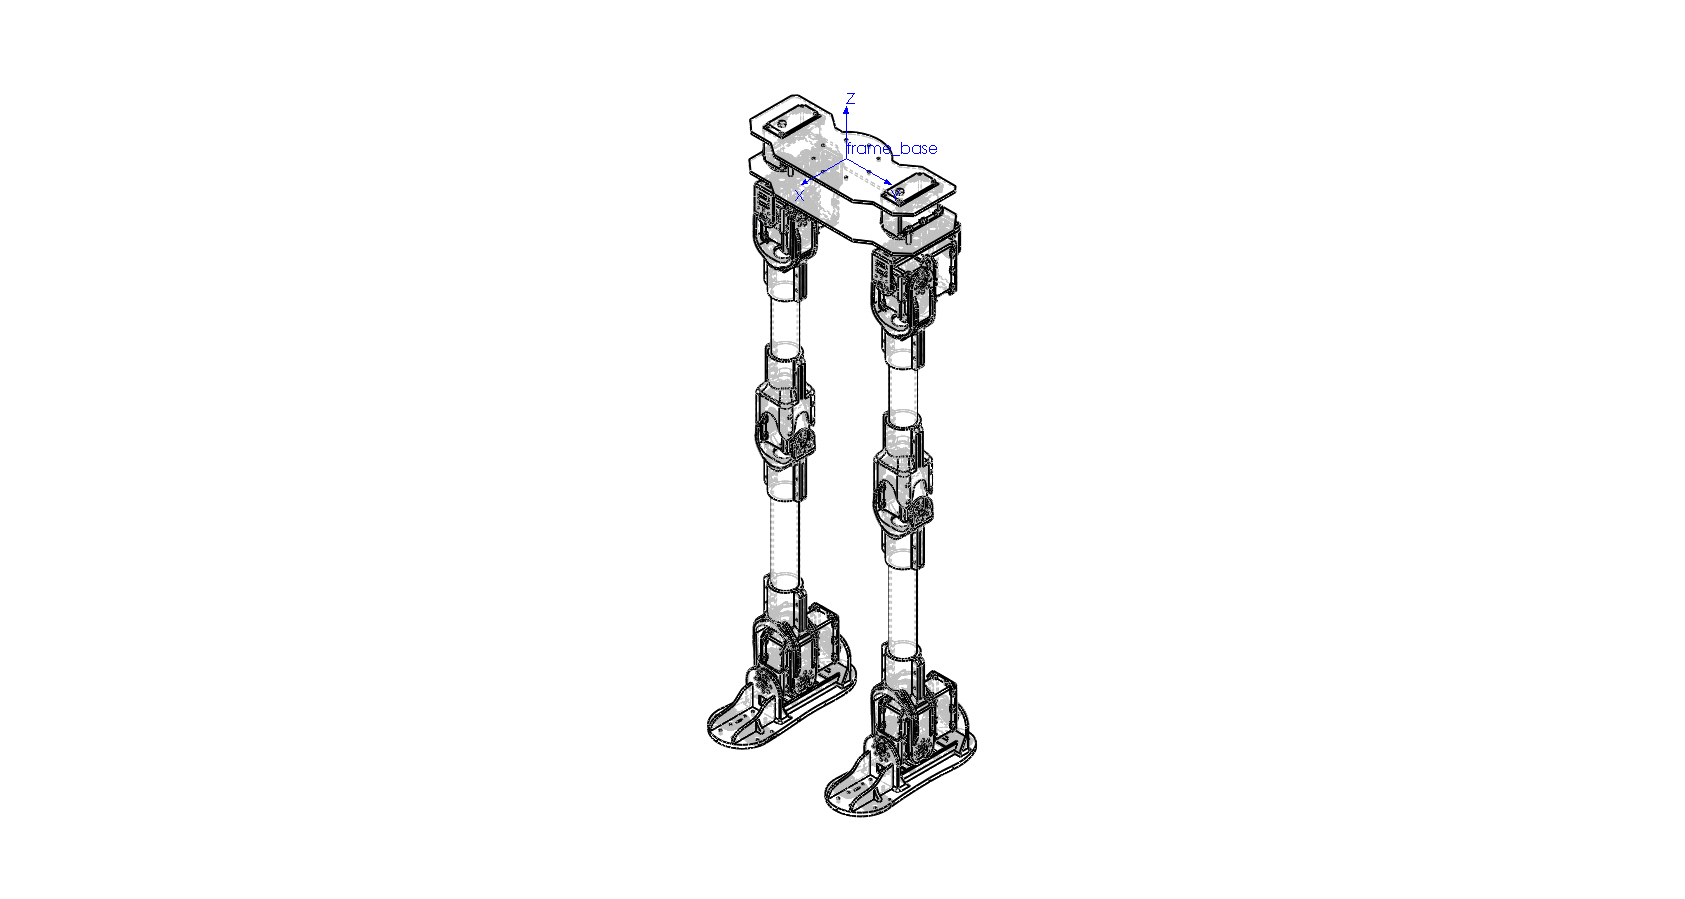
\includegraphics[width=\textwidth]{chapter3/images/uthai_dynamic_all.jpeg}
	\caption{ภาพแสดงช่วงล่างทั้งตัว}
	\label{fig:uthai_dynamic_all}
\end{figure}
\begin{table}[!ht]
	\centering
	\begin{tabular}{| c | c |}
		\hline
		Link & All Link\\
		\hline
		Mass (kg) & 3.31477475 \\
		\addprop{-0.00855772}{0.00000000}{-0.33375492}{0.28641029}{-0.00000302}{-0.00048106}{0.26207601}{-0.00061103}{0.02925799}
		\hline
	\end{tabular}
	\caption{ตารางแสดงค่าพารามิเตอร์ทั้งตัว}
	\label{tab:uthai_dynamic_all}
\end{table}


\newcommand{\adddynamicprop}[6]{
	\clearpage
	\subsubsection*{#1}
	\begin{figure}[!ht]
		\centering
		\includegraphics[width=\textwidth]{chapter3/images/{#2}.jpeg}
		\caption{ภาพแสดงก้านต่อ #1}
	\end{figure}
	\begin{table}[!ht]
		\begin{subtable}[b]{0.45\textwidth}
			\centering
			\begin{tabular}{| c | c |}
				\hline
				Link & #3\\
				\hline
				Mass (kg) & #4\\
				\addprop#5
				\hline
			\end{tabular}
			\caption{DH Parameter}
		\end{subtable}
		\begin{subtable}[b]{0.45\textwidth}
			\centering
			\begin{tabular}{| c | c |}
				\hline
				Link & #3\\
				\hline
				Mass (kg) & #4\\
				\addprop#6
				\hline
			\end{tabular}
			\caption{URDF}
		\end{subtable}
		\caption{ตารางแสดงค่าพารามิเตอร์ #1}
	\end{table}
	}
%{header name}{file name}{link name}{mass}
%{{comXdh}{comYdh}{comZdh}{Ixxdh}{Ixydh}{Ixzdh}{Iyydh}{Iyzdh}{Izzdh}}
%{{comXurdf}{comYurdf}{comZurdf}{Ixxurdf}{Ixyurdf}{Ixzurdf}{Iyyurdf}{Iyzurdf}{Izzurdf}}

\adddynamicprop{Right Hip Yaw}{uthai_dynamic_rhy}{r\_hip\_yaw}{0.09100000}
{{0.00000000}{0.02864983}{-0.02500000}{0.00014158}{0.00000000}{0.00000000}{0.00014316}{0.00000000}{0.00002022}}
{{0.00000000}{-0.02500000}{-0.00735017}{0.00014158}{0.00000000}{0.00000000}{0.00002022}{0.00000000}{0.00014316}}

\adddynamicprop{Left Hip Yaw}{uthai_dynamic_lhy}{l\_hip\_yaw}{0.09100000}
{{0.00000000}{0.02864983}{-0.02500000}{0.00014158}{0.00000000}{0.00000000}{0.00014316}{0.00000000}{0.00002022}}
{{0.00000000}{0.02500000}{-0.00735017}{0.00014158}{0.00000000}{0.00000000}{0.00002022}{0.00000000}{0.00014316}}

\adddynamicprop{Right Hip Roll}{uthai_dynamic_rhr}{r\_hip\_roll}{0.34300000}
{{0.01526237}{0.02152630}{0.00000000}{0.00026846}{0.00000219}{-0.00000081}{0.00014760}{0.00000000}{0.00032448}}
{{0.00000000}{-0.01526237}{-0.02652630}{0.00032448}{0.00000081}{0.00000000}{0.00026846}{0.00000219}{0.00014760}}

\adddynamicprop{Left Hip Roll}{uthai_dynamic_lhr}{l\_hip\_roll}{0.34300000}
{{0.01526237}{0.02152630}{0.00000000}{0.00026846}{0.00000219}{-0.00000081}{0.00014760}{0.00000000}{0.00032448}}
{{0.00000000}{-0.01526237}{-0.02652630}{0.00032448}{0.00000081}{0.00000000}{0.00026846}{0.00000219}{0.00014760}}

\adddynamicprop{Right Hip Pitch}{uthai_dynamic_rhp}{r\_hip\_pitch}{0.31800000}
{{-0.07862011}{0.00000000}{0.00000000}{0.00011525}{0.00000000}{0.00000078}{0.00254669}{0.00000000}{0.00250848}}
{{0.22137989}{0.00000000}{0.00000000}{0.00011525}{0.00000000}{0.00000078}{0.00254669}{0.00000000}{0.00250848}}

\adddynamicprop{Left Hip Pitch}{uthai_dynamic_lhp}{l\_hip\_pitch}{0.31800000}
{{-0.07862011}{0.00000000}{0.00000000}{0.00011525}{0.00000000}{0.00000078}{0.00254669}{0.00000000}{0.00250848}}
{{0.22137989}{0.00000000}{0.00000000}{0.00011525}{0.00000000}{0.00000078}{0.00254669}{0.00000000}{0.00250848}}

\adddynamicprop{Right Knee Pitch}{uthai_dynamic_rkp}{r\_knee\_pitch}{0.13800000}
{{-0.15211782}{0.00000000}{0.00000000}{0.00011525}{0.00000000}{0.00000000}{0.00127592}{0.00000000}{0.00124960}}
{{0.16288218}{0.00000000}{0.00000000}{0.00005794}{0.00000000}{0.00000000}{0.00127592}{0.00000000}{0.00124960}}

\adddynamicprop{Left Knee Pitch}{uthai_dynamic_lkp}{l\_knee\_pitch}{0.13800000}
{{-0.15211782}{0.00000000}{0.00000000}{0.00011525}{0.00000000}{0.00000000}{0.00127592}{0.00000000}{0.00124960}}
{{0.16288218}{0.00000000}{0.00000000}{0.00005794}{0.00000000}{0.00000000}{0.00127592}{0.00000000}{0.00124960}}

\adddynamicprop{Right Ankle Pitch}{uthai_dynamic_rap}{r\_ankle\_pitch}{0.33138738}
{{-0.01526237}{0.00000000}{-0.02152630}{0.00025937}{0.00000000}{0.00000079}{0.00031349}{0.00000000}{0.00014261}}
{{-0.01526237}{0.02152630}{0.00000000}{0.00025937}{0-0.00000212}{0.00000079}{0.00014261}{0.00000000}{0.00031349}}

\adddynamicprop{Left Ankle Pitch}{uthai_dynamic_lap}{l\_ankle\_pitch}{0.33138738}
{{-0.01526237}{0.00000000}{-0.02152630}{0.00025937}{0.00000000}{0.00000079}{0.00031349}{0.00000000}{0.00014261}}
{{-0.01526237}{0.02152630}{0.00000000}{0.00025937}{0-0.00000212}{0.00000079}{0.00014261}{0.00000000}{0.00031349}}

\adddynamicprop{Right Ankle Roll}{uthai_dynamic_rar}{r\_ankle\_roll}{0.10500000}
{{-0.01454118}{-0.00034576}{-0.00019548}{0.00034591}{-0.00000857}{-0.00000013}{0.00004813}{-0.00000120}{0.00032705}}
{{0.03625882}{-0.00019548}{0.00034576}{0.00034591}{-0.00000013}{0.00000857}{0.00032705}{0.00000120}{0.00004813}}

\adddynamicprop{Left Ankle Roll}{uthai_dynamic_lar}{l\_ankle\_roll}{0.10500000}
{{-0.01454118}{-0.00034576}{-0.00019548}{0.00034591}{-0.00000857}{-0.00000013}{0.00004813}{-0.00000120}{0.00032705}}
{{0.03625882}{-0.00019548}{0.00034576}{0.00034591}{-0.00000013}{0.00000857}{0.00032705}{0.00000120}{0.00004813}}
